\chapter{Vrac -Bis }

Suite du Vrac. Regroupe plut\^ot des  bribes de documentation interne
eLiSe .

%-------------------------------------------------------------------
%-------------------------------------------------------------------
%-------------------------------------------------------------------

\section{Utilisation des foncteurs compil\'es}

On retrace ici le (long \dots) chemin qui conduit de l'utilisation
finale d'un foncteur jusqu'\`a la modification d'un syst\`eme (L2 ou L1).
Il s'agit d'extrait de code avec plein de coupures.

\subsection {Fili\`ere non indexee}

{\small
\begin{verbatim}
void  cEqObsRotVect::AddObservation (...)
{
    mN2.SetEtat(aDir2/euclid(aDir2)); ....
    mSet.AddEqFonctToSys(mFoncEqResidu,aPds,WithD2);

}

REAL cSetEqFormelles::AddEqFonctToSys ( const tContFcteur & aCont ...)
{
   VAddEqFonctToSys(aFonct,aPds,WithDerSec);
}

const std::vector<REAL> & cSetEqFormelles::VAddEqFonctToSys (cElCompiledFonc * aFonct)
{
    aFonct->SetCoordCur(mAlloc.ValsVar()); // Met les val courrantes
    aFonct->SetValDer();   // Fait le calcul
    aFonct->AddDevLimOrd1ToSysSurRes(*mSys,aPds,true); // Transfert a la matrice
}

void cElCompiledFonc::AddDevLimOrd1ToSysSurRes
     (cGenSysSurResol & aSys,REAL aPds,bool EnPtsCur)
{
     AddContrainteEqSSR(false,aPds,aSys,EnPtsCur);
}

// Peut etre appelee par AddDevLimOrd1ToSysSurRe, mais aussi pour mettre
// des contraintes
void cElCompiledFonc::AddContrainteEqSSR
     (bool contr,REAL aPds,cGenSysSurResol & aSys,bool EnPtsCur)
{
   // met les valeurs des derivees dans mRealDer qui, apparemment
   // est un tableau ayant la meme taille que le systeme global !
   for ( aD ...)
       aSys.GSSR_AddNewEquation(aPds,&(mRealDer[aD][0]),aB);
}

void cGenSysSurResol::GSSR_AddNewEquation(REAL aPds,REAL * aL,REAL aB)
{
     V_GSSR_AddNewEquation(aPds,aL,aB);
}

  // Ensuite il y a differente variante, en L2 ca donne
void L2SysSurResol::V_GSSR_AddNewEquation(REAL aPds,REAL * aCoeff,REAL aB)
{
    AddEquation(aPds,aCoeff,aB);
}

void L2SysSurResol::AddEquation(REAL aPds,REAL * aCoeff,REAL aB)
{
    // selectionne (! enfin ...) les coeffs non nuls dans une table d'indexe
    L2SysSurResol::V_GSSR_AddNewEquation_Indexe(VInd,aPds,&VALS[0],aB);
}

// En L1 ca donne simplement

void SystLinSurResolu::V_GSSR_AddNewEquation(REAL aPds,REAL * aCoeff,REAL aB)
{
     PushEquation(aCoeff,aB,aPds);
}


\end{verbatim}
}


Cette fili\`ere est tr\`es lourde, cependant elle est indispensable en $L_1$, puisque
chaque \'equation doit \^etre repr\'esent\'ee explicitement et de mani\`ere compl\`ete.


\subsection {Fili\`ere indexee}

Elle est utilis\'ee par les foncteurs ayant un tres grand nombre d'inconnues
et (par consequent) des matrices creuses. Par exemple dans
{\tt src/photogram/phgr\_cGridIncImageMnt.cpp}?


{\small
\begin{verbatim}
void cGridIncImageMnt::OneStepRegulD2 (REAL aPds)
{
    ..
     pSetIncs->AddEqIndexeToSys(pRegD2,aPds/4,mIncs);
}

const std::vector<REAL> & cSetEqFormelles::AddEqIndexeToSys
   ( cElCompiledFonc * aFonct, REAL aPds, const std::vector<INT>  & aVInd)
{
    aFonct->SVD_And_AddEqSysSurResol(... ValVar() ...);
}

void cElCompiledFonc::SVD_And_AddEqSysSurResol
     (
	   const std::vector<INT> & aVInd,
	   REAL aPds,
	   REAL *       Pts,
	   cGenSysSurResol & aSys,
	   bool EnPtsCur
      )
{
   // Si oui le systeme aSys sait utiliser des directement des
   // matrice
      bool UseMat = aSys.GSSR_UseEqMatIndexee();

    ...
      if (UseMat)
      {
	   double ** aDM = aMat.data();
	   double  * aDF = aFLin.data();

	   aSys.GSSR_EqMatIndexee(aVInd,aPds,aDM,aDF,aCste);
      }
      else
      {
	  aSys.GSSR_AddNewEquation_Indexe(aVInd,aPds,&(mCompDer[aD][0]),aB);;
      }
}

  GSSR_UseEqMatIndexee :
     - vrai pour L2SysSurResol (matrice pleine)
     - faux pour cGenSysSurResol (donc pour L1 qui en derive sans redef)
     - vrai pour cFormQuadCreuse  (donc cElMatCreuseMap et cElMatCreuseStrFixe)

Par ailleur GSSR_AddNewEquation_Indexe , plante en L1.
\end{verbatim}
}

Optimisation a faire pour les grandes aeros :

\begin{itemize}
   \item   switcher, sans doute a partir de AddEqFonctToSys, vers le
   mode indexe;
    \item sauf si le system ne le supporte pas ! Donc par ex L1;
\end{itemize}


\section{Communication avec les syst\`emes sur-contraints}

\subsection{Convention d'\'ecritures}

Soit un ensemble d'\'equations d'observations :

\begin{equation}
   F^j(X)- O^j = 0;
\end{equation}

Un foncteur correpond a une lin\'erisation de  ces equations.  On
regroupe plusieur \'equations en un seul foncteur, lorsqu'il y a une
synergie permettant de mettre en commun les calcul (cas courant, projection
image en $x$ et $y$).  A VOIR : PEUT ON GAGNER DU TEMPS EN FACTORISANT TOUTE
LES OBSERVARION D'UNE PROJECTION SUR UNE MEME CAMERA.

Si on lin\'earise l'\'equation en $X_0$, on a :

\begin{equation}
   F^j(X_0) + \sum{\frac{\partial F^j}{\partial X_k} \delta_k} - O^j = 0;
\end{equation}

En notant :

\begin{equation}
      D^j_k= \frac{\partial F^j}{\partial X_k} = {\tt mCompDer[j][k]}
\end{equation}
\begin{equation}
      V^j =  F^j(X_0) - O^j = {\tt mVal[j]}
\end{equation}

On a l'\'equation lin\'eaire  dont les para\`etres sont calcul\'es dans le foncteur:

\begin{equation}
    \sum{ D^j_k \delta_k}  + V^j = 0;
\end{equation}


Dans l'interface des syst\`emes lin\'eaire, le m\'ethod {\tt GSSR\_AddNewEquation(P,A,B)}
correspond \`a l'observation :

\begin{equation}
    (\sum{ A_k X_k} = B ) * P;
\end{equation}


C'est pour cela que dans {\tt AddContrainteEqSSR} on a $B=-V$.

A priori, dans toutes ces \'equations, l'inconnue est directement un delta
par rapport au point courant (param\`etre {\tt EnPtsCur} vaut {\tt true}).
Si ce n'\'etait pas le cas,  les inconnues seraient $x_k$ et les  \'equation
deviendraient :

\begin{equation}
   F^j(X_0) + \sum{\frac{\partial F^j}{\partial X_k} (x_k-{X_0}_k} - O^j = 0;
\end{equation}

Soit  :

\begin{equation}
    \sum{D^j_k x_k} =   \sum{D^j_k {X_0}_k} -V;
\end{equation}

D'o\`u le code extrait de {\tt cElCompiledFonc::AddContrainteEqSSR} :

\begin{verbatim}
   REAL aB = -mVal[aD];
    ...
	 aB +=  mCompDer[aD][aIC] * mCompCoord[aIC]
\end{verbatim}


\subsection{UseEqMatIndexee}


Si le syst\`eme d'\'equation l'autorise, on va \'ecrire directemnt un forme
quadratique . Chaque \'equation :

\begin{equation}
    P (^t L  X =  B)
\end{equation}

Apporte une contribution :

\begin{equation}
    P (^t L  X -  B) ^2  = P (^t X (^tLL)X  -2B^tL X + B^2)
\end{equation}

\section{Mesh computation}

Commands are:

\begin{itemize}
\item {\tt Malt} with ZoomF=4 (or 8 if you tweak the code...) or use meshlab to downsample point cloud after Nuage2Ply and MergePly (clustered vertex sampling, with cell size = 0,25 \%, and average parameter)
\item {\tt Nuage2Ply} with Normale=5 option: computes local normal for each point and writes a .ply file with X Y Z NX NY NZ format.
\item {\tt MergePly} writes one ply file from multiple ply files
\item {\tt PoissonRecon} {\it from Michael Kazhdan and Matthew Bolitho}, computes a mesh from the previous ply file (binary can be found in binaire-aux/)

\end{itemize}

\subsection{Command {\tt Nuage2Ply} :}

"Normale" parameters indicates the window size to compute normal: should be 3, 5, 7, etc...

\subsection{Command {\tt MergePly} :}

MergePly command concats several ply files.

\begin{verbatim}
mm3d MergePly
*****************************
*  Help for Elise Arg main  *
*****************************
Mandatory unnamed args :
  * string :: {Full Name (Dir+Pattern)}
Named args :
  * [Name=Out] string
  * [Name=Bin] INT :: {Generate Binary or Ascii (Def=true, Binary)}
\end{verbatim}

\subsection{Example}

\begin{verbatim}
mm3d Nuage2Ply NuageImProf_Geom-Im-5564_Etape_5.xml Normale=5 Out=Fic0.ply
mm3d Nuage2Ply NuageImProf_Geom-Im-5581_Etape_5.xml Normale=5 Out=Fic1.ply
mm3d Nuage2Ply NuageImProf_Geom-Im-5588_Etape_5.xml Normale=5 Out=Fic2.ply

mm3d MergePly .*ply Out=merged.ply Normale=1

PoissonRecon --in merged.ply --out result_poisson --depth 10
\end{verbatim}

\begin{verbatim}
PoissonRecon
Usage: PoissonRecon
	--in  <input points>
	[--out <ouput triangle mesh>]
	[--voxel <ouput voxel grid>]
	[--depth <maximum reconstruction depth>=8]
		 Running at depth d corresponds to solving on a 2^d x 2^d x 2^d
		 voxel grid.
	[--fullDepth <full depth>=5]
		 This flag specifies the depth up to which the octree should be complete.
	[--voxelDepth <depth at which to extract the voxel grid>=<depth>]
	[--cgDepth <conjugate-gradients depth>=0]
		 The depth up to which a conjugate-gradients solver should be used.
	[--scale <scale factor>=1.100000]
		 Specifies the factor of the bounding cube that the input
		 samples should fit into.
	[--samplesPerNode <minimum number of samples per node>=1.000000]
		 This parameter specifies the minimum number of points that
		 should fall within an octree node.
	[--pointWeight <interpolation weight>=4.000000]
		 This value specifies the weight that point interpolation constraints are
		 given when defining the (screened) Poisson system.
	[--iters <iterations>=8]
		 This flag specifies the (maximum if CG) number of solver iterations.
		 This parameter specifies the number of threads across which
		 the solver should be parallelized.
	[--confidence]
		 If this flag is enabled, the size of a sample's normals is
		 used as a confidence value, affecting the sample's
		 constribution to the reconstruction process.
	[--nWeights]
		 If this flag is enabled, the size of a sample's normals is
		 used as to modulate the interpolation weight.
	[--polygonMesh]
		 If this flag is enabled, the isosurface extraction returns polygons
		 rather than triangles.
	[--density]
		 If this flag is enabled, the sampling density is written out with the vertices.
	[--double]
		 If this flag is enabled, the reconstruction will be performed with double-precision floats.
	[--verbose]
		 If this flag is enabled, the progress of the reconstructor will be output to STDOUT.
\end{verbatim}
For more information on Misha Khazdan's code: \url{http://www.cs.jhu.edu/~misha/Code/PoissonRecon/}



\chapter{Various formula}

I put here different formula that may be useful to understand some part of MicMac. As it's purely utilitarian, I do it the fast way by
scanning the paper version.

\section{Space resection}


As the code for computation of space resection from $3$ GCP is a bit tricky, I have summarized the main
computation on figure~\ref{Not:ResSpace}. This notation should be compatible with the variable
of class {\tt cNewResProfChamp<Type>} defined in {\tt src/photogram/phgr\_low\_level.cpp}


\begin{figure}
\begin{tabular}{|c|}
   \hline \hline
   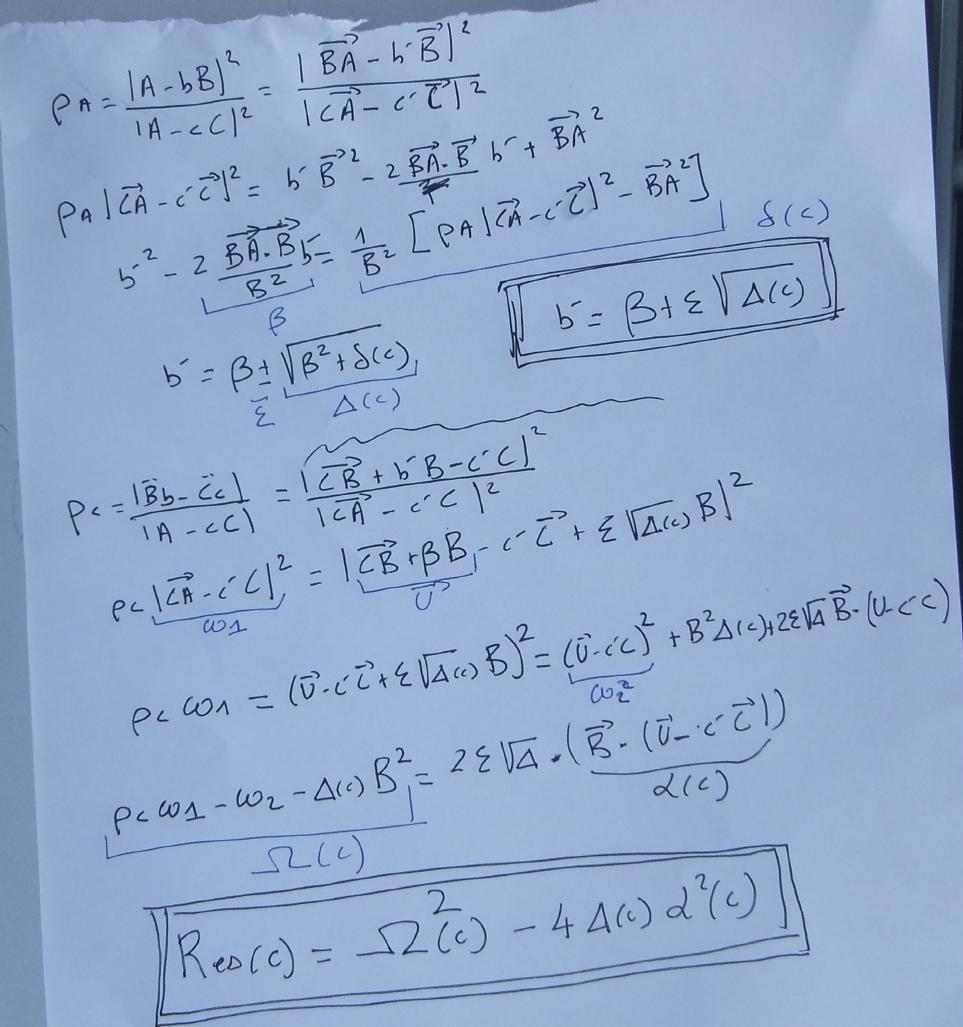
\includegraphics[width=160mm]{FIGS/Formules/NotattionSpace.JPG}
\end{tabular}
\label{Not:ResSpace}
\caption{Notation for space resection}
\end{figure}


\section{Stretching (etirement)}

I put her the justification of stretching formula in function {\tt cZBuffer::BasculerUnTriangle} :

\begin{figure}
\begin{tabular}{|c|}
   \hline \hline
   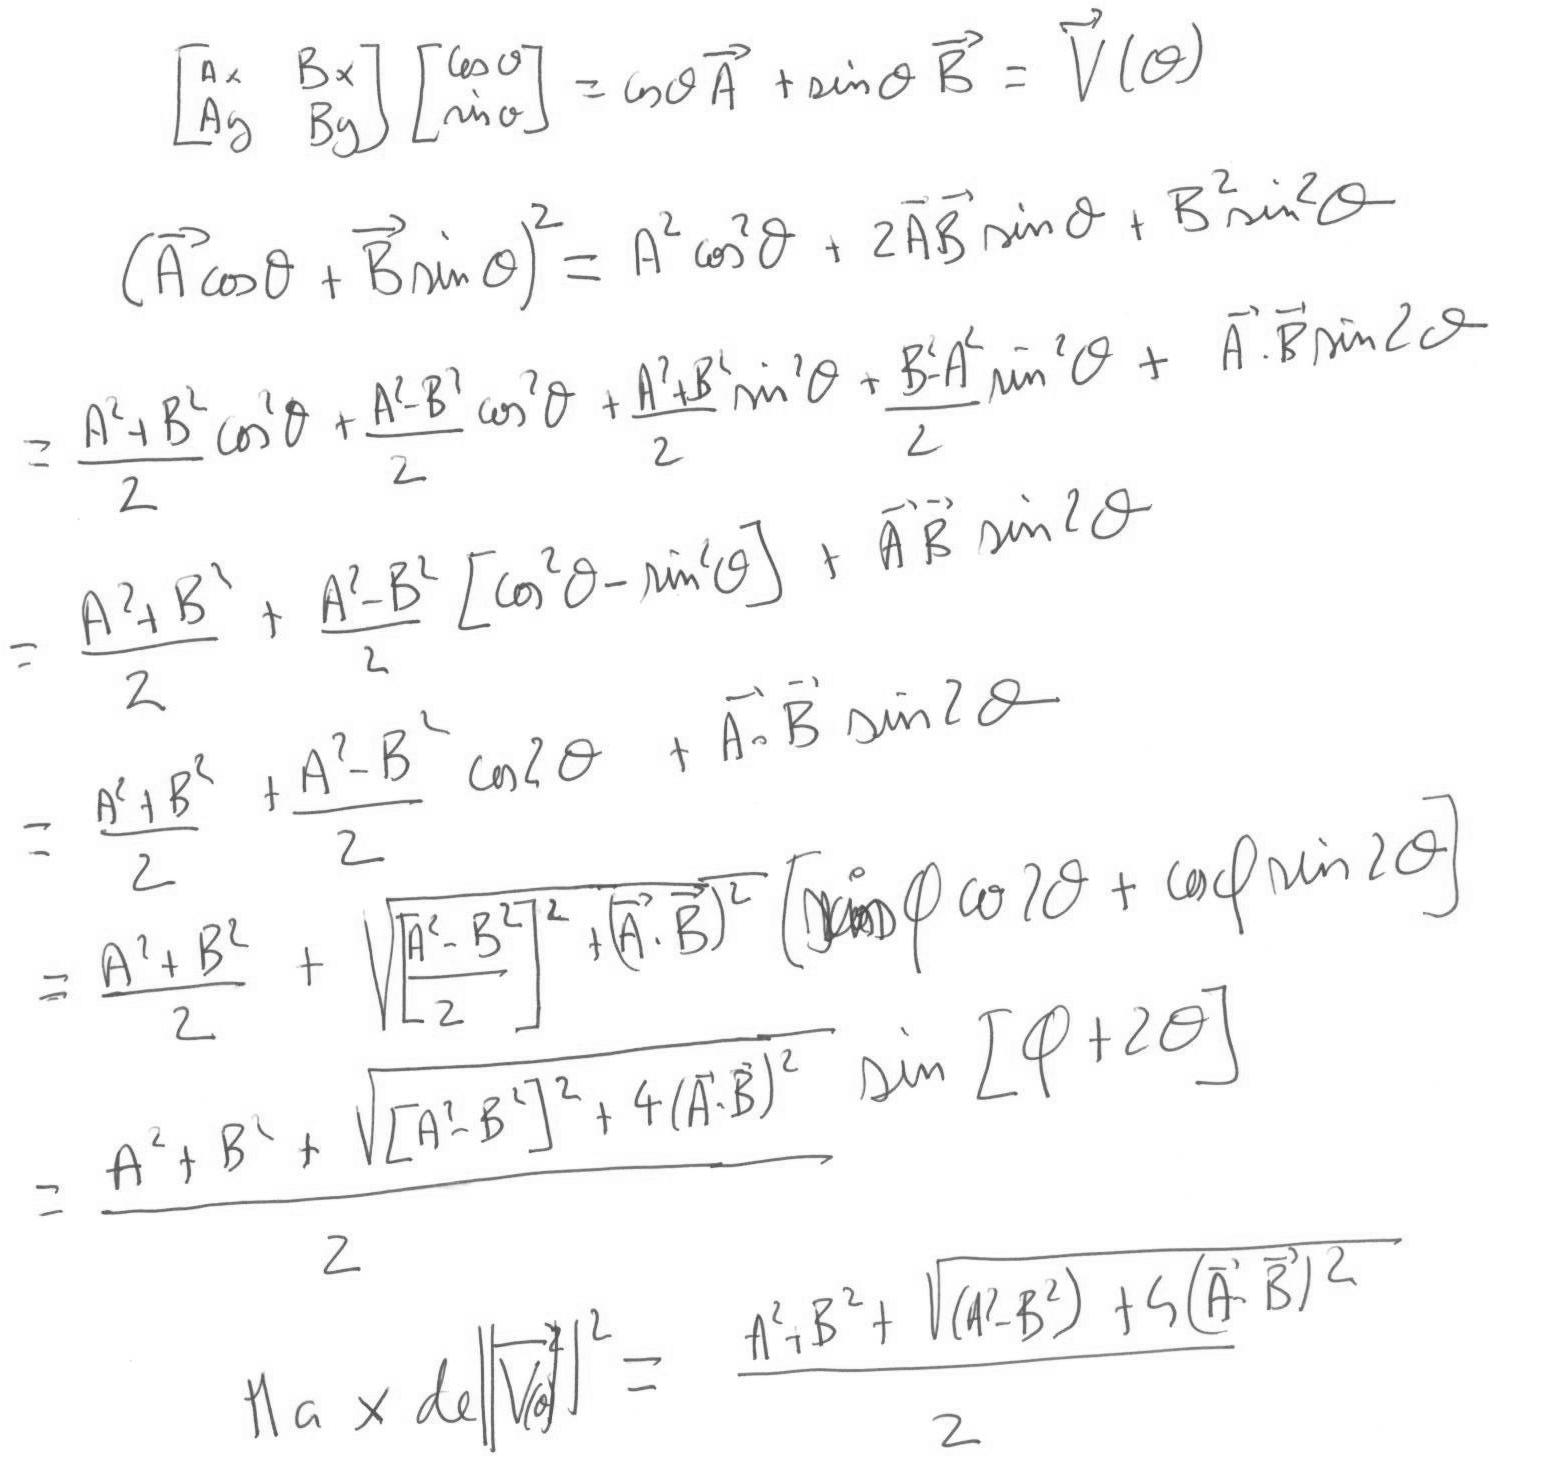
\includegraphics[width=160mm]{FIGS/Formules/CalcEtir.JPG}
\end{tabular}
\label{Not:CalcEtir}
\caption{Computation of stretching-etirement formula}
\end{figure}


